\documentclass{article}
\usepackage{graphicx}
\pagestyle{empty}

\begin{document}
%%%%%%%%%%%%%%%%%%%%%%%%%%%%%%
\begin{center}
Si(001)$2\times 1$ reconstruction\\
$\chi^{xxx}_{\mathrm{2\times 1}}\ne 0$\\
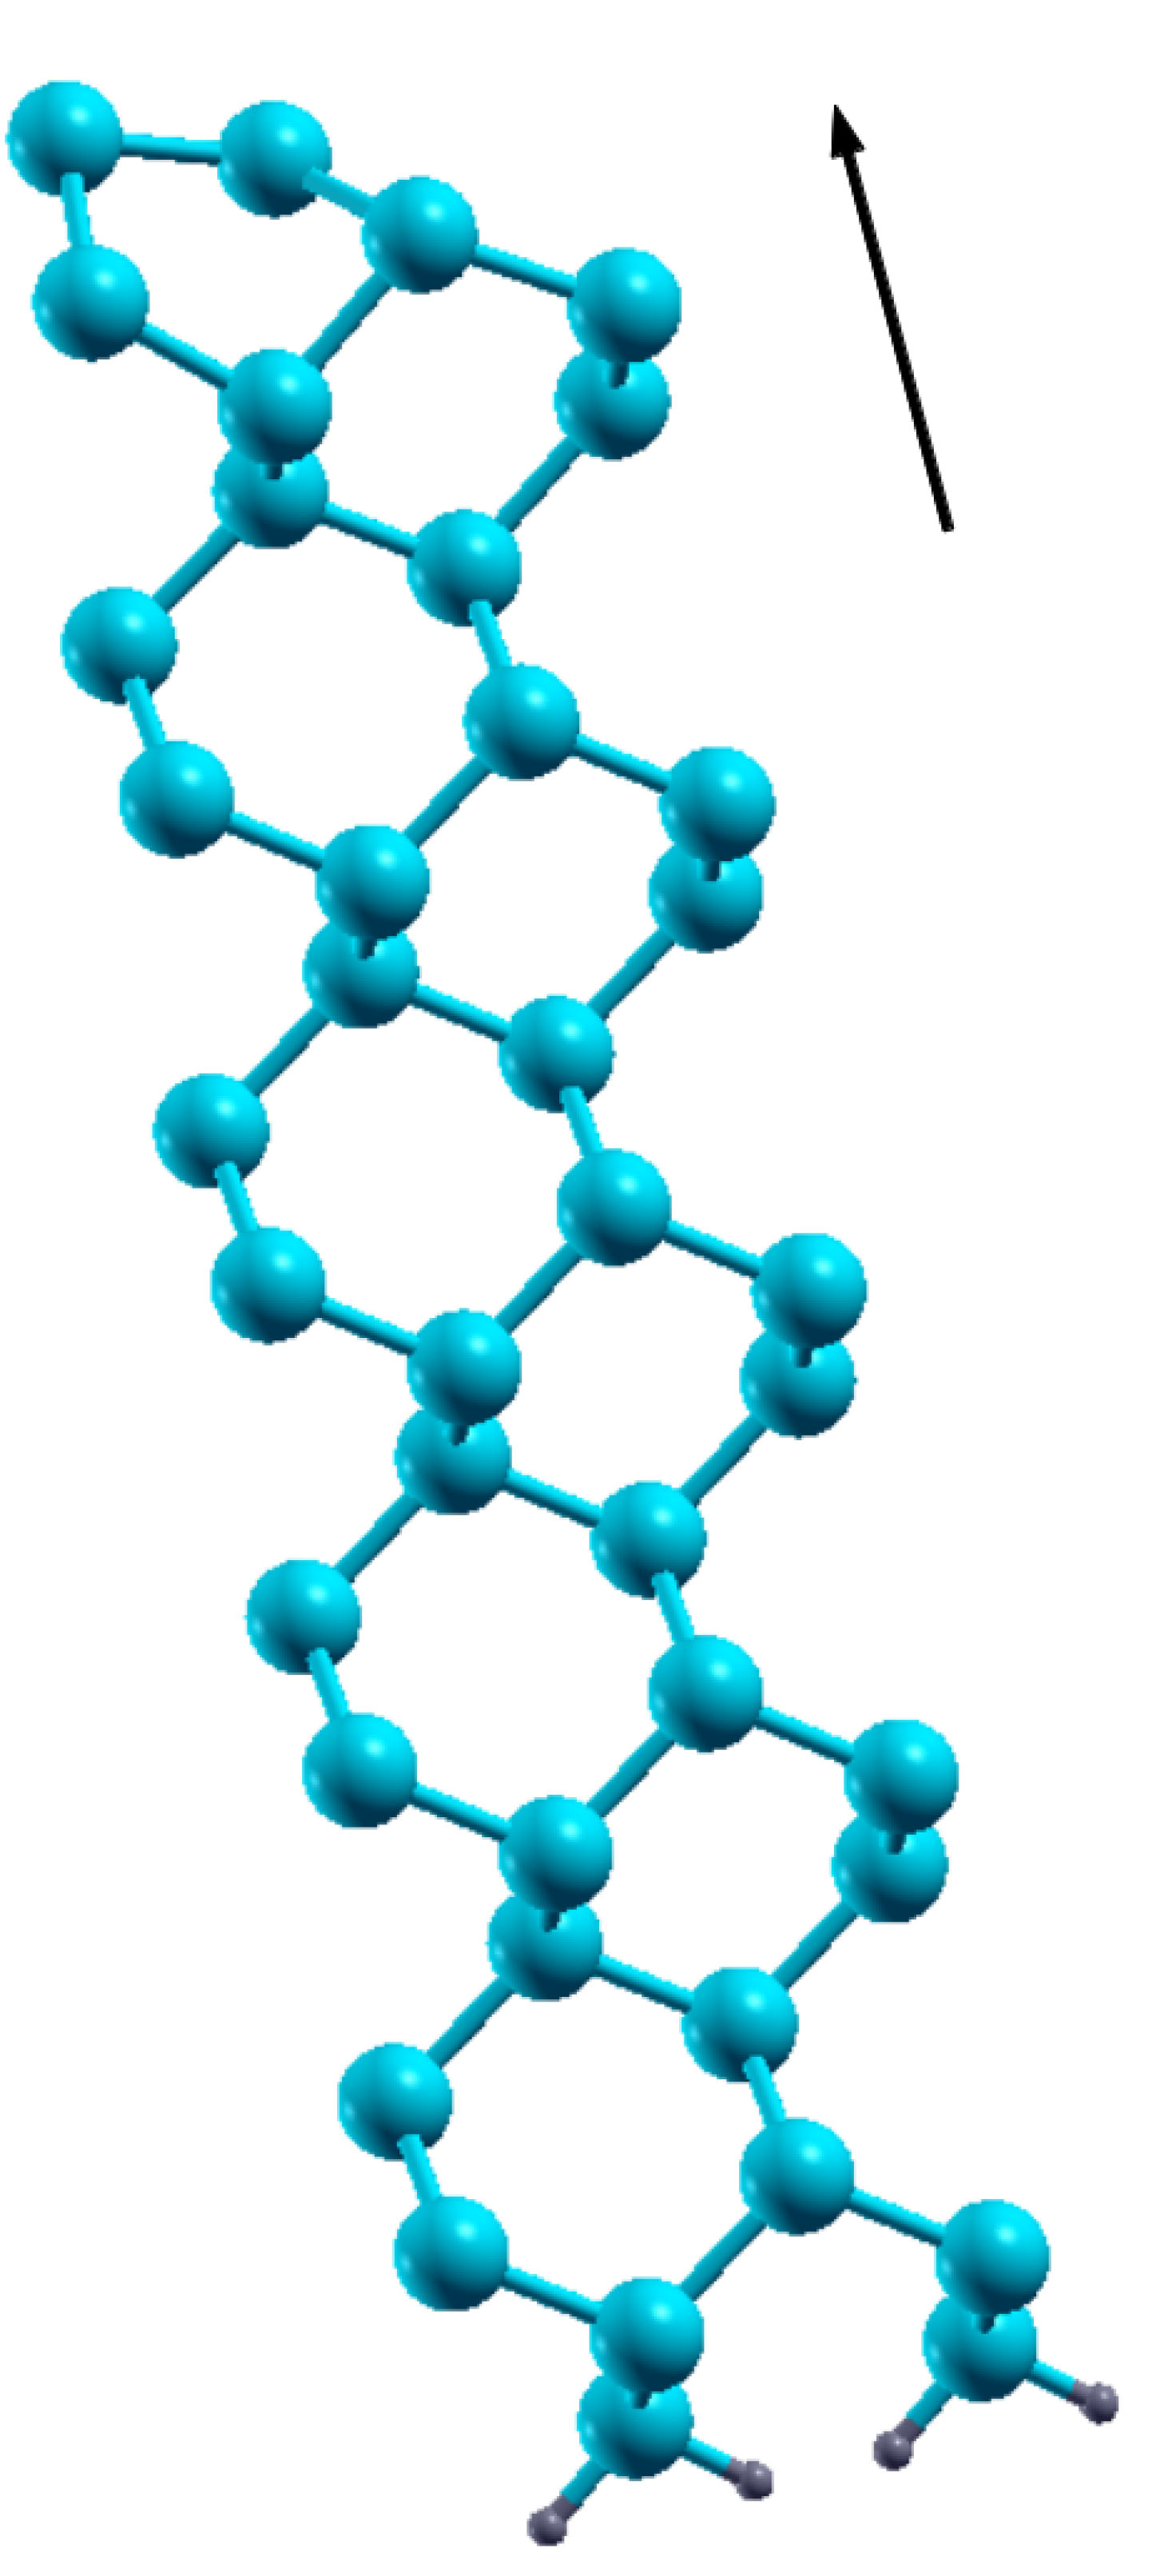
\includegraphics[scale=.25]{Si2x1bare.jpg}\\
H-terminated $\Rightarrow\chi^{xxx}_{\mathrm{H}}= 0$
\begin{picture}(5,20) 
\put(-30,190){$z$-axis}
\put(-140,150){${\mathcal{C}}^{\ell}(z) = 1$}
\put(-140,101.5){\line(5,1){150}}
\put(-140,50){${\mathcal{C}}^{\ell}(z) = 0$}
\end{picture}
\end{center}
%%%%%%%%%%%%%%%%%%%%%%%%%%%%%%
\end{document}
